\documentclass[12pt]{beamer}
\usepackage{../Estilos/BeamerFC}
\usepackage{tabulary}
\usepackage{../Estilos/ColoresLatex}
\usepackage{courier}
\usepackage{listingsutf8}
\usepackage{listings}
\usepackage{xcolor}
\usepackage{textcomp}
\usepackage{color}
\definecolor{deepblue}{rgb}{0,0,0.5}
\definecolor{brown}{rgb}{0.59, 0.29, 0.0}
\definecolor{OliveGreen}{rgb}{0,0.25,0}
% \usepackage{minted}

\DeclareCaptionFont{white}{\color{white}}
\DeclareCaptionFormat{listing}{\colorbox{gray}{\parbox{0.98\textwidth}{#1#2#3}}}
\captionsetup[lstlisting]{format=listing,labelfont=white,textfont=white}
\renewcommand{\lstlistingname}{Código}


\definecolor{Code}{rgb}{0,0,0}
\definecolor{Keywords}{rgb}{255,0,0}
\definecolor{Strings}{rgb}{255,0,255}
\definecolor{Comments}{rgb}{0,0,255}
\definecolor{Numbers}{rgb}{255,128,0}

\makeatletter

\newif\iffirstchar\firstchartrue
\newif\ifstartedbyadigit
\newif\ifprecededbyequalsign

\newcommand\processletter
{%
  \ifnum\lst@mode=\lst@Pmode%
    \iffirstchar%
        \global\startedbyadigitfalse%
      \fi
      \global\firstcharfalse%
    \fi
}

\newcommand\processdigit
{%
  \ifnum\lst@mode=\lst@Pmode%
      \iffirstchar%
        \global\startedbyadigittrue%
      \fi
      \global\firstcharfalse%
  \fi
}

\lst@AddToHook{OutputOther}%
{%
  \lst@IfLastOtherOneOf{=}
    {\global\precededbyequalsigntrue}
    {}%
}

\lst@AddToHook{Output}%
{%
  \ifprecededbyequalsign%
      \ifstartedbyadigit%
        \def\lst@thestyle{\color{orange}}%
      \fi
    \fi
  \global\firstchartrue%
  \global\startedbyadigitfalse%
  \global\precededbyequalsignfalse%
}

\lstset{ 
language=Python,                % choose the language of the code
basicstyle=\footnotesize\ttfamily,       % the size of the fonts that are used for the code
numbers=left,                   % where to put the line-numbers
numberstyle=\scriptsize,      % the size of the fonts that are used for the line-numbers
stepnumber=1,                   % the step between two line-numbers. If it is 1 each line will be numbered
numbersep=5pt,                  % how far the line-numbers are from the code
backgroundcolor=\color{white},  % choose the background color. You must add \usepackage{color}
showspaces=false,               % show spaces adding particular underscores
showstringspaces=false,         % underline spaces within strings
showtabs=false,                 % show tabs within strings adding particular underscores
frame=single,   		% adds a frame around the code
tabsize=2,  		% sets default tabsize to 2 spaces
captionpos=t,   		% sets the caption-position to bottom
breaklines=true,    	% sets automatic line breaking
breakatwhitespace=false,    % sets if automatic breaks should only happen at whitespace
escapeinside={| |},  % if you want to add a comment within your code
stringstyle =\color{OliveGreen},
otherkeywords={as, np.array, np.concatenate, np.linspace, linspace, interpolate.interp1d, kind, plt.plot, .copy, np.arange, np.cos, np.pi, lw, ls, label, splrep, splev, plt.legend, loc, plt.title, plt.ylim, plt.show, sign, math.ceil, math.log, np.sqrt, np.exp, np.zeros, plt.xlabel, plt.ylabel, plt.xlim, np.identity, random, np.dot, np.outer, np.diagonal },             % Add keywords here
keywordstyle = \color{blue},
commentstyle = \color{darkcerulean},
identifierstyle = \color{black},
literate=%
         {á}{{\'a}}1
         {é}{{\'e}}1
         {í}{{\'i}}1
         {ó}{{\'o}}1
         {ú}{{\'u}}1
%
%keywordstyle=\ttb\color{deepblue}
%fancyvrb = true,
}

\lstdefinestyle{FormattedNumber}{%
    literate={0}{{\textcolor{red}{0}}}{1}%
             {1}{{\textcolor{red}{1}}}{1}%
             {2}{{\textcolor{red}{2}}}{1}%
             {3}{{\textcolor{red}{3}}}{1}%
             {4}{{\textcolor{red}{4}}}{1}%
             {5}{{\textcolor{red}{5}}}{1}%
             {6}{{\textcolor{red}{6}}}{1}%
             {7}{{\textcolor{red}{7}}}{1}%
             {8}{{\textcolor{red}{8}}}{1}%
             {9}{{\textcolor{red}{9}}}{1}%
             {.0}{{\textcolor{red}{.0}}}{2}% Following is to ensure that only periods
             {.1}{{\textcolor{red}{.1}}}{2}% followed by a digit are changed.
             {.2}{{\textcolor{red}{.2}}}{2}%
             {.3}{{\textcolor{red}{.3}}}{2}%
             {.4}{{\textcolor{red}{.4}}}{2}%
             {.5}{{\textcolor{red}{.5}}}{2}%
             {.6}{{\textcolor{red}{.6}}}{2}%
             {.7}{{\textcolor{red}{.7}}}{2}%
             {.8}{{\textcolor{red}{.8}}}{2}%
             {.9}{{\textcolor{red}{.9}}}{2}%
             {\ }{{ }}{1}% handle the space
         ,%
          %mathescape=true
          escapeinside={__}
          }



\usetheme{Warsaw}
\usecolortheme{seahorse}
%\useoutertheme{default}
\setbeamercovered{invisible}
% or whatever (possibly just delete it)
\setbeamertemplate{section in toc}[sections numbered]
\setbeamertemplate{subsection in toc}[subsections numbered]
\setbeamertemplate{subsection in toc}{\leavevmode\leftskip=3.2em\rlap{\hskip-2em\inserttocsectionnumber.\inserttocsubsectionnumber}\inserttocsubsection\par}
\setbeamercolor{section in toc}{fg=blue}
\setbeamercolor{subsection in toc}{fg=blue}
\setbeamercolor{frametitle}{fg=blue}
\setbeamertemplate{caption}[numbered]

\setbeamertemplate{footline}
\beamertemplatenavigationsymbolsempty
\setbeamertemplate{headline}{}


\makeatletter
\setbeamercolor{section in foot}{bg=gray!30, fg=black!90!orange}
\setbeamercolor{subsection in foot}{bg=blue!30}
\setbeamercolor{date in foot}{bg=black}
\setbeamertemplate{footline}
{
  \leavevmode%
  \hbox{%
  \begin{beamercolorbox}[wd=.333333\paperwidth,ht=2.25ex,dp=1ex,center]{section in foot}%
    \usebeamerfont{section in foot} \insertsection
  \end{beamercolorbox}%
  \begin{beamercolorbox}[wd=.333333\paperwidth,ht=2.25ex,dp=1ex,center]{subsection in foot}%
    \usebeamerfont{subsection in foot}  \insertsubsection
  \end{beamercolorbox}%
  \begin{beamercolorbox}[wd=.333333\paperwidth,ht=2.25ex,dp=1ex,right]{date in head/foot}%
    \usebeamerfont{date in head/foot} \insertshortdate{} \hspace*{2em}
    \insertframenumber{} / \inserttotalframenumber \hspace*{2ex} 
  \end{beamercolorbox}}%
  \vskip0pt%
}
\makeatother

\makeatletter
\patchcmd{\beamer@sectionintoc}{\vskip1.5em}{\vskip0.8em}{}{}
\makeatother

%\newlength{\depthofsumsign}
%\setlength{\depthofsumsign}{\depthof{$\sum$}}
% \newcommand{\nsum}[1][1.4]{% only for \displaystyle
%     \mathop{%
%         \raisebox
%             {-#1\depthofsumsign+1\depthofsumsign}
%             {\scalebox
%                 {#1}
%                 {$\displaystyle\sum$}%
%             }
%     }
% }
\def\scaleint#1{\vcenter{\hbox{\scaleto[3ex]{\displaystyle\int}{#1}}}}
\def\scaleoint#1{\vcenter{\hbox{\scaleto[3ex]{\displaystyle\oint}{#1}}}}
\def\bs{\mkern-12mu}

\usefonttheme{serif}

\title{\large{Tema 1 - Errores y artimética de punto flotante}}
\author{M. en C. Gustavo Contreras Mayén}
\date{ }

\begin{document}
\maketitle

\section*{Contenido}
\frame[allowframebreaks]{\frametitle{Contenido} \tableofcontents[currentsection, hideallsubsections]}

\section{Eficiencia}
\frame[allowframebreaks]{\tableofcontents[currentsection, hideothersubsections]}
\subsection{Definición}

\begin{frame}
\frametitle{Eficiencia}
\emph{En todo momento debemos evitar que todo algoritmo sea inestable}. \pause Si existieran varios métodos para evaluar una misma función, entonces conviene utilizar aquel que sea más eficiente, es decir, más rápido.
\\
\bigskip
\pause
\textcolor{blue}{Hay que aprovechar al máximo los recursos: hardware, software, algoritmos, para resolver problemas más complejos y no para resolver peor problemas simples.}
\end{frame}
\begin{frame}
\frametitle{Ahorro en las operaciones}
Por ejemplo, para calcular $x**4$ para un $x$ dado, no es buena idea calcular $x**4.0$ (exponente en punto flotante).
\\
\bigskip
\pause
La mejor idea consiste en economizar el cálculo en dos pasos:
\pause
\begin{eqnarray*}
\begin{aligned}
x^{2} &= x * x \\ \pause
x^{4} &= x^{2} * x^{2}
\end{aligned}
\end{eqnarray*}
y no un producto $x^{4} = x * x * x * x$
\end{frame}
\begin{frame}
\frametitle{Ejemplo: Evaluación de polinomios}
Supongamos que queremos evaluar el polinomio:
\pause
\begin{align*}
P (x) = 2 + 4 \, x - 5 \, x^{2} + 2 \, x^{3} - 6 \, x^{4} + 8 \, x^{5} + 10 \, x^{6}
\end{align*}
\pause
Contando con que cada potencia de exponente $k$ entero como $k-1$ productos, tendríamos que el total de productos para evaluar en forma directa es:
\pause
\begin{align*}
1 + 2 + 3 + 4 + 5 + 6 = 21
\end{align*}
Además de seis sumas.
\end{frame}
\begin{frame}
\frametitle{Mejora para el cálculo}
Una mejora en el algoritmo , es calcular primero las potencias de forma sucesiva:
\pause
\begin{eqnarray*}
\begin{aligned}
x^{2} &= x * x \\ \pause
x^{3} &= x * x^{2} \\ \pause
x^{4} &= x * x^{3} \\ \pause
x^{5} &= x * x^{4} \\ \pause
x^{6} &= x * x^{5}
\end{aligned}
\end{eqnarray*}
\end{frame}
\begin{frame}
\frametitle{Mejora para el cálculo}
De tal forma que se añade un producto por cada potencia, para un total de productos:
\pause
\begin{align*}
1 + 2 + 2 + 2 + 2 + 2 = 11
\end{align*}
\end{frame}
\begin{frame}
\frametitle{Mejorando el cálculo de un polinomio}
Con el polinomio:
\pause
\begin{align*}
P (x)= 2 + 4 \, x - 5 \, x^{2} + 2 \, x^{3} - 6 \, x^{4} + 8 \, x^{5} + 10 \, x^{6}
\end{align*}
\pause
podemos \emph{mejorar} el algoritmo de la siguiente manera:
\pause
\begin{align*}
P(x) = 2 + x \left\lbrace 4 + x \left( -5 + x \left[ 2 + x \left(-6 +x \left\lbrace 8+x*10 \right\rbrace \right) \right] \right) \right\rbrace
\end{align*}
\end{frame}
\begin{frame}
\frametitle{Pasos necesarios para la evaluación}
Para evaluar un polinomio de grado $n$ en el que ninguno de los coeficientes es cero, se necesitan:
\pause
\begin{table}
\centering
\begin{tabular}{l l}
Productos & Método \\ \hline
$\dfrac{n \, (n + 1)}{2}$ & Primero \\ \hline
$2 \, n - 1$ & Segundo \\ \hline
$n$ & Tercero \\ \hline
\end{tabular}
\end{table}
\pause
Antes de escribir una línea de código, hay que revisar la manera en que podemos optimizar la solución del problema.
\end{frame}

\subsection{El método de Horner}

\begin{frame}
\frametitle{El método de Horner}
Dado el polinomio:
\pause
\begin{align*}
P (x) = a_{0} + a_{1} \, x + \ldots + a_{n} \, x^{n} \hspace{1cm} a_{n} \neq 0
\end{align*}
\pause
La evaluación de $P (x)$ para cierto valor de $x = z$ se puede realizar en $n$ pasos mediante:
\end{frame}
\begin{frame}
\frametitle{El método de Horner}
La evaluación de $P (x)$ para cierto valor de $x = z$ se puede realizar en $n$ pasos mediante:
\begin{eqnarray*}
\begin{aligned}
b_{n} &= a_{n} \\ \pause
b_{n-1} &= a_{n-1} + z * b_{n} \\ \pause
b_{n-2} &= a_{n-2} + z * b_{n-1} \\ \pause
\vdots \\ \pause
b_{0} &= a_{0} + z * b_{1}
\end{aligned}
\end{eqnarray*}
\end{frame}
\begin{frame}
\frametitle{Pseudocódigo}
\setbeamercolor{item projected}{bg=black,fg=white}
\setbeamertemplate{enumerate items}{%
\usebeamercolor[bg]{item projected}%
\raisebox{1.5pt}{\colorbox{bg}{\color{fg}\footnotesize\insertenumlabel}}%
}
\begin{enumerate}[<+->]
\item $b_{n} = a_{n}$
\item repetir mientras $n > 0$
\item $n = n - 1$
\item $b = a_{n} + z * b$
\item volver al paso 2
\item $p (z) = b$
\end{enumerate}
\end{frame}

\subsection{Ejercicio}

\begin{frame}
\frametitle{Completa la siguiente tabla}
\begin{align*}
P (x) = 2 + 4 \, x - 5 \, x^{2} + 2 \, x^{3} - 6 \, x^{4} + 8 \, x^{5} + 10 \, x^{6}
\end{align*}
Evalúa con un algoritmo en \python{} el polinomio $P (x)$ en:
\begin{table}
\renewcommand{\arraystretch}{0.8}
\centering
\begin{tabular}{c | c}
$x$ & $P (x)$ \\ \hline
$-1.5$ & \\ \hline
$-0.65$ & \\ \hline
$0.1$ & \\ \hline
$1.4$ & \\ \hline
$2.87$ & \\ 
\end{tabular}
\end{table}
\end{frame}

\subsection*{Extendiendo la respuesta}

\begin{frame}
\frametitle{Extendiendo la respuesta al problema}
\setbeamercolor{item projected}{bg=ao,fg=white}
\setbeamertemplate{enumerate items}{%
\usebeamercolor[bg]{item projected}%
\raisebox{1.5pt}{\colorbox{bg}{\color{fg}\footnotesize\insertenumlabel}}%
}
\begin{enumerate}[<+->]
\item ¿Cómo resolver el problema usando una función? 
\item ¿Mostrando una tabla con formato de salida?
\item ¿Una gráfica que muestre $P (x)$ y un conjunto de datos evaluados?
\item ¿Evaluar el error relativo?
\end{enumerate}
\end{frame}
\begin{frame}
\frametitle{Extendiendo la respuesta al problema}
Ya contamos con las herramientas necesarias para extender la respuesta al problema, en nuestro código podemos agregar funciones, ajustar formatos de salida en los resultados, graficar el polinomio y los puntos (o un conjunto diferente de puntos), y obtener el error relativo. Basta con que le dediquemos un poco más de tiempo.
\end{frame}
\begin{frame}
\frametitle{Pasos a resolver}
\setbeamercolor{item projected}{bg=cadetblue,fg=lava}
\setbeamertemplate{enumerate items}{%
\usebeamercolor[bg]{item projected}%
\raisebox{1.5pt}{\colorbox{bg}{\color{fg}\footnotesize\insertenumlabel}}%
}
\begin{enumerate}[<+->]
\item Conviene definir una función que resuelva la evaluación del método de Horner.
\item Para obtener el error relativo, se debe de evaluar el polinomio y considerar que los valores obtenidos, son los valores exactos.
\item Comparamos los resultados mediante una gráfica que represente los dos resultados de la evaluación.
\end{enumerate}
\end{frame}
\begin{frame}[fragile]
\frametitle{Evaluando el polinomio $P (x)$}
En un primer momento pensaremos implementar una función en \python{} que nos evalúe directamente los puntos de la lista, algo del tipo:
\pause
\begin{lstlisting}[caption=Evluación directa del polinomio]
def eval_polinomio(x):
    valor = 2 + 4 * x - 5 * x**2 + 2 * x**3 - 6 * x**4 + \
    8 * x**5 + 10 * x**6
    return valor
\end{lstlisting}
\end{frame}
\begin{frame}[fragile]
\frametitle{Resultado válido}
El resultado que nos devuelve la función cumple lo necesario, bastaría indicar los puntos $x$ en los que queremos evaluar el polinomio:
\pause
\begin{lstlisting}[caption=Evaluando los puntos]
x0 = [-1.5, -0.65, 0.1, 1.4, 2.87]

for i in x0:
    eval_polinomio(i)
\end{lstlisting}
\end{frame}
\begin{frame}
\frametitle{Simplificando con python las tareas}
Veamos la manera en simplificar con \python{} las tareas de definir un polinomio $P (x)$ y evaluar varios puntos $x_{0}$:
\\
\bigskip
\pause
Usaremos la librería \funcionazul{NumPy} y un módulo para trabajar con \emph{polinomios}.
\end{frame}

\subsection{NumPy}

\begin{frame}
\frametitle{La Librería \texttt{NumPy}}
\texttt{NumPy} es la librería fundamental para la computación científica en Python.
\\
\bigskip
\pause
Es una biblioteca de \python{} que proporciona un objeto de matriz multidimensional: \textbf{\texttt{narray}}, así como varios objetos derivados (como vectores y matrices).
\end{frame}
\begin{frame}
\frametitle{La Librería \texttt{NumPy}}
Así como una variedad de rutinas para operaciones rápidas en matrices, que incluyen \pause manipulación matemática, \pause lógica, \pause de formas, \pause clasificación, \pause selección, \pause E/S., \pause transformadas discretas de Fourier, \pause álgebra lineal básica, \pause operaciones estadísticas básicas, \pause simulación aleatoria y mucho más.
\end{frame}
\begin{frame}
\frametitle{Definiendo el polinomio}
Ocuparemos de \texttt{numpy} el módulo \texttt{polynomial}:
{\fontsize{12}{12} \selectfont
\texttt{numpy.polynomial.polynomial}}
\\
\bigskip
\pause
Con la siguiente función construimos el polinomio.
\end{frame}
\begin{frame}
\frametitle{Definiendo el polinomio}
Definimos un polinomio con el objeto:
\\
\pause
{\fontsize{12}{12} \selectfont
\texttt{Polynomial(coef)}}
\\
\pause
donde \texttt{coef} es un arreglo de los coeficientes, deben de indicarse de manera creciente: $([1, 2, 3])$ devuelve:
\pause
\begin{align*}
1 + 2 \, x + 3 \, x**2
\end{align*}
\end{frame}
\begin{frame}[fragile]
\frametitle{El polinomio $p (x)$}
Una vez definido el polinomio, podemos evaluar un punto en el mismo, indicando como argumento:
\pause
\begin{lstlisting}[caption=Definiendo el polinomio p(x)]
coef = [2, 4, -5, 2, -6, 8, 10]

p = np.polynomial.polynomial.Polynomial(coef)
print(p(1))    
\end{lstlisting}
Esto nos evalúa un punto, ¿podremos evaluar más puntos en un solo paso?
\end{frame}
\begin{frame}
\frametitle{Evaluando varios puntos al mismo tiempo}
Para evaluar en un polinomio varios puntos, es necesario cambiar la función, \pause ahora usarmos \texttt{polyval}.
\\
\bigskip
\pause
\texttt{polyval(lista\_puntos, coef)}
\setbeamercolor{item projected}{bg=lilac,fg=white}
\setbeamertemplate{enumerate items}{%
\usebeamercolor[bg]{item projected}%
\raisebox{1.5pt}{\colorbox{bg}{\color{fg}\footnotesize\insertenumlabel}}%
}
\begin{enumerate}[<+->]
\item \texttt{lista\_puntos} es el arreglo con los puntos en donde queremos evaluar el polinomio.
\item \texttt{coef} son los coeficientes del polinomio.
\end{enumerate}
\end{frame}
\begin{frame}[fragile]
\frametitle{Evaluando varios puntos al mismo tiempo}
\begin{lstlisting}[caption=Evaluando los puntos con polyval]
x0 = [-1.5, -0.65, 0.1, 1.4, 2.87]

valores = np.polynomial.polynomial.polyval(x0, coef)
print(valores)
\end{lstlisting}
\pause
Tenemos de regreso un objeto \funcionazul{array} con cada valor evaluado en el polinomio.
\end{frame}
\begin{frame}
\frametitle{$P (x)$ evaluado en los puntos anteriores}
\begin{table}
\centering
%\begin{tabular}{S[table-format=1.2] | S[table-format=4.5] }
\begin{tabular}{c | c}
$x$ & $P (x)$ \\ \hline
$-1.5$ & $0.78125$ \\ \hline
$-0.65$ & $-4.50683$ \\ \hline
$0.1$ & $2.35149$ \\ \hline
$1.4$ & $98.55968$ \\ \hline
$2.87$ & $6758.70245$
\end{tabular}
\end{table}
\end{frame}

\subsection{Algortimo de Horner}

\begin{frame}[fragile]
\frametitle{El método de Horner}
El sigiuente paso es implementar el método de Horner dentro de una función:
\begin{lstlisting}[caption=El método de Horner]
def funcion_Horner(x):
    # Anota tu codigo aqui.
\end{lstlisting}
\end{frame}
\begin{frame}[fragile]
\frametitle{Calculando el error relativo}
Se necesita estimar el error relativo entre el cálculo con la función \textoazul{eval} y el método de Horner:
\begin{lstlisting}[caption=Función para el error relativo]
def error_relativo(arg1, arg2):
    # Anota tu codigo aqui.
\end{lstlisting}
\end{frame}
\begin{frame}[fragile]
\frametitle{Rutina de graficación}
Por último, nos resta agregar una rutina de graficación:
\begin{lstlisting}[caption=Rutina de graficación]
import matplotlib.pyplot as plt

plt.plot(x1, funcion_eval, label=u'Evaluación Polinomio')
plt.plot(x0, funcion_horner, 'or', label='Método de Horner')
\end{lstlisting}
\end{frame}
\begin{frame}
\frametitle{Gráfica obtenida}
Luego de completar el código, debemos de obtener una gráfica como la que a continuación se muestra.
\end{frame}
\begin{frame}[fragile]
\frametitle{Gráfica obtenida}
\begin{figure}
    \centering
    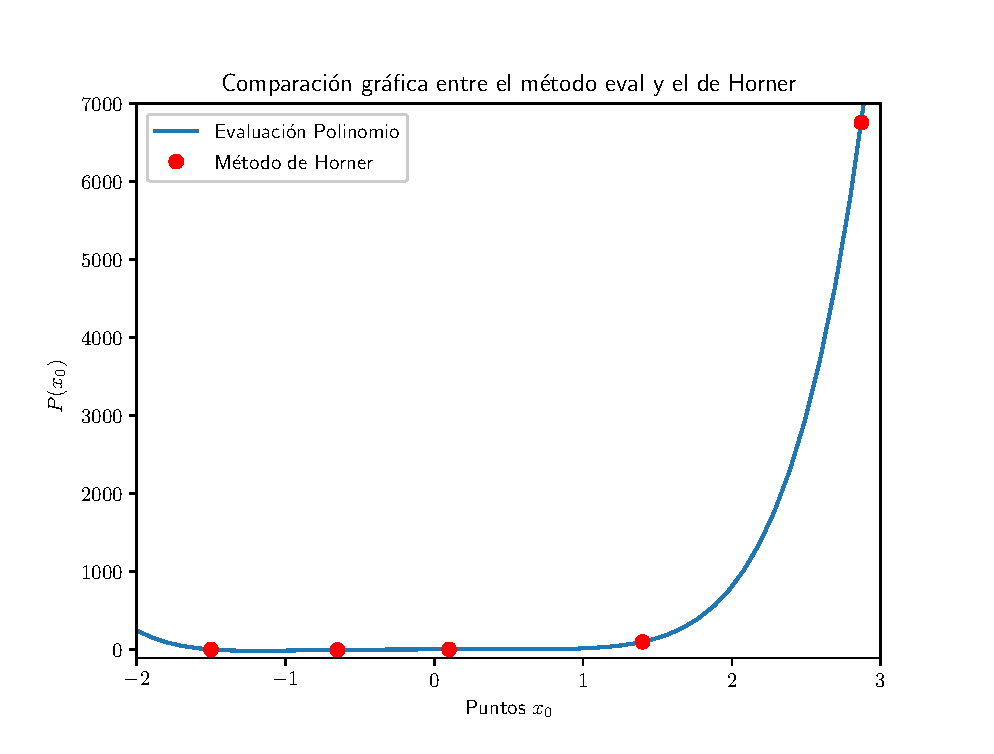
\includegraphics[scale=0.6]{Imagenes/Plot_Metodo_Horner_01.eps} 
\end{figure}
\end{frame}
\begin{frame}[fragile]
\frametitle{Resultado gráfico más completo}
En la gráfica se muestra un conjunto de datos que se evalúan y posteriormente con la función (en línea continua) se compara, podemos ver que los resultados son prácticamente los mismos.
\end{frame}


\end{document}